\chapter{Investigating the Molecular Mechanisms of Tension-dependent Re-localisation of Shugoshin}

\section{Introduction}
Centromere executes its function of coordinating chromosome segregation partially by controlling the subcellular location of critical regulators. A remarkable example is the tension-dependent re-localisation of shugoshin. 

To be segregated into different daughter cells later, sister chromatids need to be bipolarly attached to the spindle in mitosis or meiosis II, which is called bi-orientation \citep{Tanaka2010Kinetochore-microtubuleBi-orientation}. Bi-oriented sister chromatids come under tension due to the counteraction between the resistance of cohesion and the pulling of microtubules. Cells sense a lack of tension and destabilise erroneous microtubule-kinetochore attachment, a process termed error correction, meanwhile delaying cell cycle progression until tension is generated \citep{Nicklas1997HowChromosomes, Nicklas1994, Tanaka2010Kinetochore-microtubuleBi-orientation}. The conserved shugoshin protein family is important for the establishment of tension \citep{Watanabe2005, Clift2011, Gutierrez-Caballero2012Shugoshins:Centromere, Marston2015, Zhang2020FunctioningMitosis}. The name itself, 'guardian spirit' in Japanese, comes from its well-conserved canonical function of cohesion protection in meiosis I \citep{Lister2010Age-relatedSgo2, Llano2008Shugoshin-2Mice, Lee2008, Rattani2013Sgol2Oocytes, Marston2004a, Kitajima2004a, Katis2004, Rabitsch2004TwoII, Kerrebrock1992TheDifferentiation, Cromer2013CentromericInterkinesis, Zamariola2014SHUGOSHINsThaliana, Wang2011OsSGO1Meiosis, Hamant2005AFunctions, Ma2021MeikinI, Miyazaki2017HierarchicalI}. In vertebrates, shugoshin also protects centromeric cohesion from Wapl-mediated cohesin removal pathway in mitosis \citep{Rivera2009ShugoshinExtracts, Shintomi2009ReleasingSgo1, Huang2007, Tang2006a, McGuinness2005ShugoshinCells, Kitajima2005, Salic2004VertebrateMitosis, Liang2019ACells}. Shugoshin further assists cohesion protection by directly sequestering separase with the SAC component Mad2\citep{Rattani2013Sgol2Oocytes, Hellmuth2020Securin-independentShugoshinMAD2, Orth2011ShugoshinMad2}. Apart from cohesion protection, shugoshin additionally promotes bi-orientation by facilitating error correction \citep{Meppelink2015Shugoshin-1Bi-orientation, Huang2007, Peplowska2014, Nerusheva2014, Verzijlbergen2014, Tsukahara2010a, Yamagishi2010, Hadders2020UntanglingMitosis, Broad2020AuroraCells, Kawashima2007, Vanoosthuyse2007, Rivera2012} and, at least in yeast, contributing to the geometry of the centromeric region biased towards a shape where sister kinetochores are more easily captured by microtubules from the opposite spindle poles \citep{Indjeian2007, Haase2012Bub1Dynamics, Verzijlbergen2014, Peplowska2014, Sane2021ShugoshinDisassembly}. Despite different molecular details in various species, all these functions are implemented by shugoshin acting as an adaptor recruiting different effector proteins to the centromeric region, including PP2A-B56 \citep{Xu2009StructureInteraction, Ueki2021AMitosis}, CPC \citep{Abad2022MechanisticCPC}, MCAK \citep{Tanno2010} and condensin \citep{Verzijlbergen2014, Yahya2020}. 

Interestingly, the location of shugoshin has been found to change in response to tension across species. Human Sgo1 and Sgo2 redistribute from the inner centromere towards the kinetochore upon tension establishment in mitosis \citep{Huang2007, Lee2008, Liu2013, Asai2020}. Mouse Sgo2 follows the same pattern in meiosis II \citep{Lee2008, Gomez2007}. In budding yeast, tension removes its only shugoshin protein Sgo1 from peri-centromere \citep{Eshleman2014, Nerusheva2014, Paldi2020ConvergentPericentromeres}. Although the effect of tension has not been directly studied, locations are different between metaphase and anaphase for \textit{Drosophila} MEI-S332 (mitosis and meiosis II) and fission yeast Sgo2 (mitosis) \citep{Clarke2005, Kawashima2007}, raising the possibility that they also undergo tension-dependent re-localisation. 

Re-localisation of shugoshin is functionally relevant. It has been proposed as key to tension sensing \citep{Marston2015}. Screening in budding yeast identified Sgo1 being required to delay anaphase onset in the absence of tension \citep{Indjeian2005a}. Later, it was shown to be due to its role in preventing SAC silencing \citep{Jin2013TheAttachment}. Given the function of Sgo1 to support CPC localisation, it was reasoned that tension-dependent re-localisation of Sgo1 triggers the removal of CPC from the centromere, leading to SAC silencing \citep{Nerusheva2014}. In support of this model, artificially tethering Sgo1 to the kinetochore caused prolonged metaphase \citep{Su2021SumoylationAnaphase}. In mammals, the re-localisation is thought to inactivate cohesin protection \citep{Lee2008}. Indeed, impaired human Sgo1 re-localisation increased lagging chromosomes in anaphase \citep{Liu2013}. Besides, at least in budding yeast, the re-localisation of shugoshin might be the signal for chromosome condensation. The key condensation player condensin spreads from the centromere to chromosome arms in a tension-dependent manner \citep{Leonard2015}. As its interactor with a similar response to tension, Sgo1 potentially mediates the spread. Consistent with this idea, mitotic chromosome condensation is abolished in \textit{sgo1} mutant \citep{Kruitwagen2018}. 

It is well established across species that the SAC component Bub1 kinase at the kinetochore phosphorylates threonine 120 of histone H2A (serine 121 in yeast) around centromeric chromatin, providing a high-affinity marker for shugoshin \citep{Rivera2012, Boyarchuk2007Bub1Centromere, Williams2017Bub1Kinetochores, Kitajima2005, Perera2010, Tang2004, Fernius2007Bub1Mitosis, Kiburz2005}. Nevertheless, the localisation of shugoshin is further regulated by complicated, not fully understood, interplay of various factors through reversible PTMs. In human cells, a step-wise recruitment model of Sgo1 has been proposed \citep{Liu2013, Liu2013a, Liu2015}. Sgo1 is first recruited proximal to the kinetochore due to direct binding to nucleosomes with H2A-pT120. Pol II-mediated centromeric transcription then disengages Sgo1 from nucleosomes, allowing it to reach the inner centromere. Finally, Sgo1 phosphorylated at threonine 346 by CDK is captured by cohesin there. A number of other factors supporting shugoshin localisation have been reported in different species, including HP1 \citep{Yamagishi2008, Kang2011, Perera2010}, CPC \citep{Huang2007, Tanno2010, Rivera2012, Kawashima2007, Boyarchuk2007Bub1Centromere, Resnick2006INCENPDrosophila}, PP2A \citep{Tang2006a}, CENP-A \citep{Petty2018ConnectingCheckpoint, Eot-Houllier2018AuroraFatigue, Mishra2018BuddingChromatin} and H3 \citep{Buehl2018a, Luo2016}, while Polo kinase \citep{Clarke2005}, SET \citep{Qu2019SETSegregation, Krishnan2017Phospho-H1Mitosis}, KAT2A \citep{Petty2018ConnectingCheckpoint} and PP2A \citep{Nerusheva2014} were suggested to de-localise it. 

The mechanism of shugoshin tension-dependent re-localisation is less well understood. \cite{Nerusheva2014} attempted to address it in budding yeast, yet questions are left to be answered. It was proposed that reduced Bub1 activity at peri-centromere by tension leads to the de-phosphorylation of its substrate(s), thus resulting in the removal of Sgo1. How Bub1 activity in a particular area is regulated by tension remains to be elucidated. Due to technical difficulties, it was unable to directly monitor H2A-pS121 by that time, leaving the effect of tension on it untested. Moreover, this model predicts the existence of at least one phosphatase antagonizing Bub1. Although it was found that PP2A-B56 (Rts1 in budding yeast) negatively regulates Sgo1 enrichment at the peri-centromere, whether it is responsible for Sgo1 de-localisation is unclear. The human model emphasizes phospho-regulation of shugoshin interaction with cohesin by tension underlying its movement from the inner centromere to the kinetochore-proximal region \citep{Liu2013, Liu2015}. It is interesting to explore if this mechanism could be conserved in budding yeast as well. Besides, the exact localisation of human H2A-pT120 by IF is inconsistent in the literature, with reports arguing it covers both the inner centromere \citep{Yamagishi2010} and the kinetochore proximity or it is usually only at the latter \citep{Liu2013}. Due to the repetitive nature of human centromere, the two arguments could not be distinguished by sequence-based technology such as ChIP. Whereas budding yeast can be used to address this question for its point centromere structure. 


\nomenclature{SAC}{Spindle Assembly Checkpoint}
\nomenclature{CPC}{Chromosome Passenger Complex}
\nomenclature{PP2A}{Protein Phosphatase 2A}
\nomenclature{MCAK}{Mitotic Centromere-Associated Kinesin}
\nomenclature{SET}{SET nuclear proto-oncogene}
\nomenclature{CDK}{Cyclin-Dependent Kinase}
\nomenclature{Pol II}{RNA Polymerase II}
\nomenclature{HP1}{Heterochromatin Protein 1}
\nomenclature{KAT2A}{lysine AcetylTransferase 2A}
\nomenclature{PTM}{Post Translational Modification}
\nomenclature{ChIP}{Chromatin ImmunoPrecipitation}
\nomenclature{IF}{ImmunoFluorescence}


\section{Results}
\subsection{Whether tension pulls Bub1 away from the peri-centromere border is inconclusive}
It is unclear how tension inhibits Bub1 activity at the peri-centromere. One possibility is that kinetochore-localised Bub1 is pulled away from its substrates at the peri-centromere because of tension \citep{Nerusheva2014}. This hypothesis is further supported by the study on peri-centromeric chromatin conformation showing that tension reduces the interaction between the core centromere and peri-centromeric borders \citep{Paldi2020ConvergentPericentromeres}, where Sgo1 mainly localises revealed by ChIP-seq \citep{Verzijlbergen2014, Deng2018}. 

To test this idea, I first wanted to measure FRET between Bub1 and nucleosomes. If the hypothesis is true, the FRET signal should decrease in the presence of tension. hence, I constructed a strain bearing BUB1-mNG HTB1-mCherry and pMET-CDC20. To validate the method, cells were synchronized in G1 and released into a metaphase arrest without tension by nocodazole, as this condition is expected to give a higher FRET signal. Unfortunately, it was unable to detect any FRET signal between Bub1 and Htb1, leaving the method usable (Figure~\ref{fig:FRET}). The problem is possibly due to the low expression of Bub1 protein and the small size of budding yeast. 
\nomenclature{FRET}{Förster Resonance Energy Transfer}

\begin{figure}[htb]
  \centering
  \includesvg[width=0.6\textwidth]{figures/Bub1-mNG Htb1-mCherry FRET.svg}
  \caption[Representative image of FRET between Bub1-mNG and Htb1-mCherry of metaphase cells without tension]{Representative image of FRET between Bub1-mNG and Htb1-mCherry of metaphase cells without tension. Bleed-through from both fluorophores to the FRET channel are subtracted. }
  \label{fig:FRET}
\end{figure} 

As an alternative approach, I decided to directly measure the distance between Bub1 and peri-centromeric borders, which is expected to increase by tension. To this end, I labelled one peri-centromeric border of chromosome I using the Tet-On system, with a tetO array on the locus and tetR-tdTomato under a constitutive promoter. Cells bearing BUB1-mNG pMET-CDC20 and the labelled peri-centromeric border of chromosome I were synchronized in G1 and released into +MET media for a metaphase arrest with tension. Time-lapse live-cell imaging was performed since the G1 release. Bub1-mNG appears as one focus as cells enter the S phase, indicated by the appearance of small buds. This is due to centromere clustering in budding yeast \citep{Taddei2012StructureNucleus}. All kinetochores  are seen together as one dot under current light microscopes. Bub1-mNG then splits into two foci due to sister kinetochores separating by tension. On the other hand, tetR-tdTomato stays as one focus from the beginning of imaging. Occasionally, it splits into two foci after the separation of Bub1-mNG foci (Figure~\ref{fig:periCEN}A). The distance between Bub1-mNG and tetR-tdTomato focus $L$ was measured. After the separation of Bub1-mNG, there could be two $L$s in one cell. I arbitrarily named the shorter one as $L_{1}$ and the longer one as $L_{2}$. The inter-kinetochore distance measured from the distance between Bub1-mNG dots was used as the indicator of tension. Before Bub1-mNG separation, $L$ ranges from 0.01 to 1.19 \si{\micro\metre} with a median of 0.32 \si{\micro\metre}. After Bub1-mNG separation, $L_{1}$ and $L_{2}$ together gave a data set showing a slight increase, ranging from 0.01 to 1.24 \si{\micro\metre} with a median of 0.40 \si{\micro\metre}. However, if analysed individually, $L_{1}$ is not correlated with the inter-kinetochore distance ($R^2 = 0.03$) despite $L_{2}$ shows a moderated correlation ($R^2 = 0.59$) (Figure~\ref{fig:periCEN}B).This result suggests the distance between one of the Bub1-mNG foci and the peri-centromere border is independent of tension, arguing against the hypothesis of Bub1 being pulled further away from its substrates at the peri-centromere. Whereas the other Bub1-mNG focus does become further, favouring the hypothesis. Therefore, whether tension pulls Bub1 away from the peri-centromere border is inconclusive. 


\begin{figure}[htbp]
  \centering
  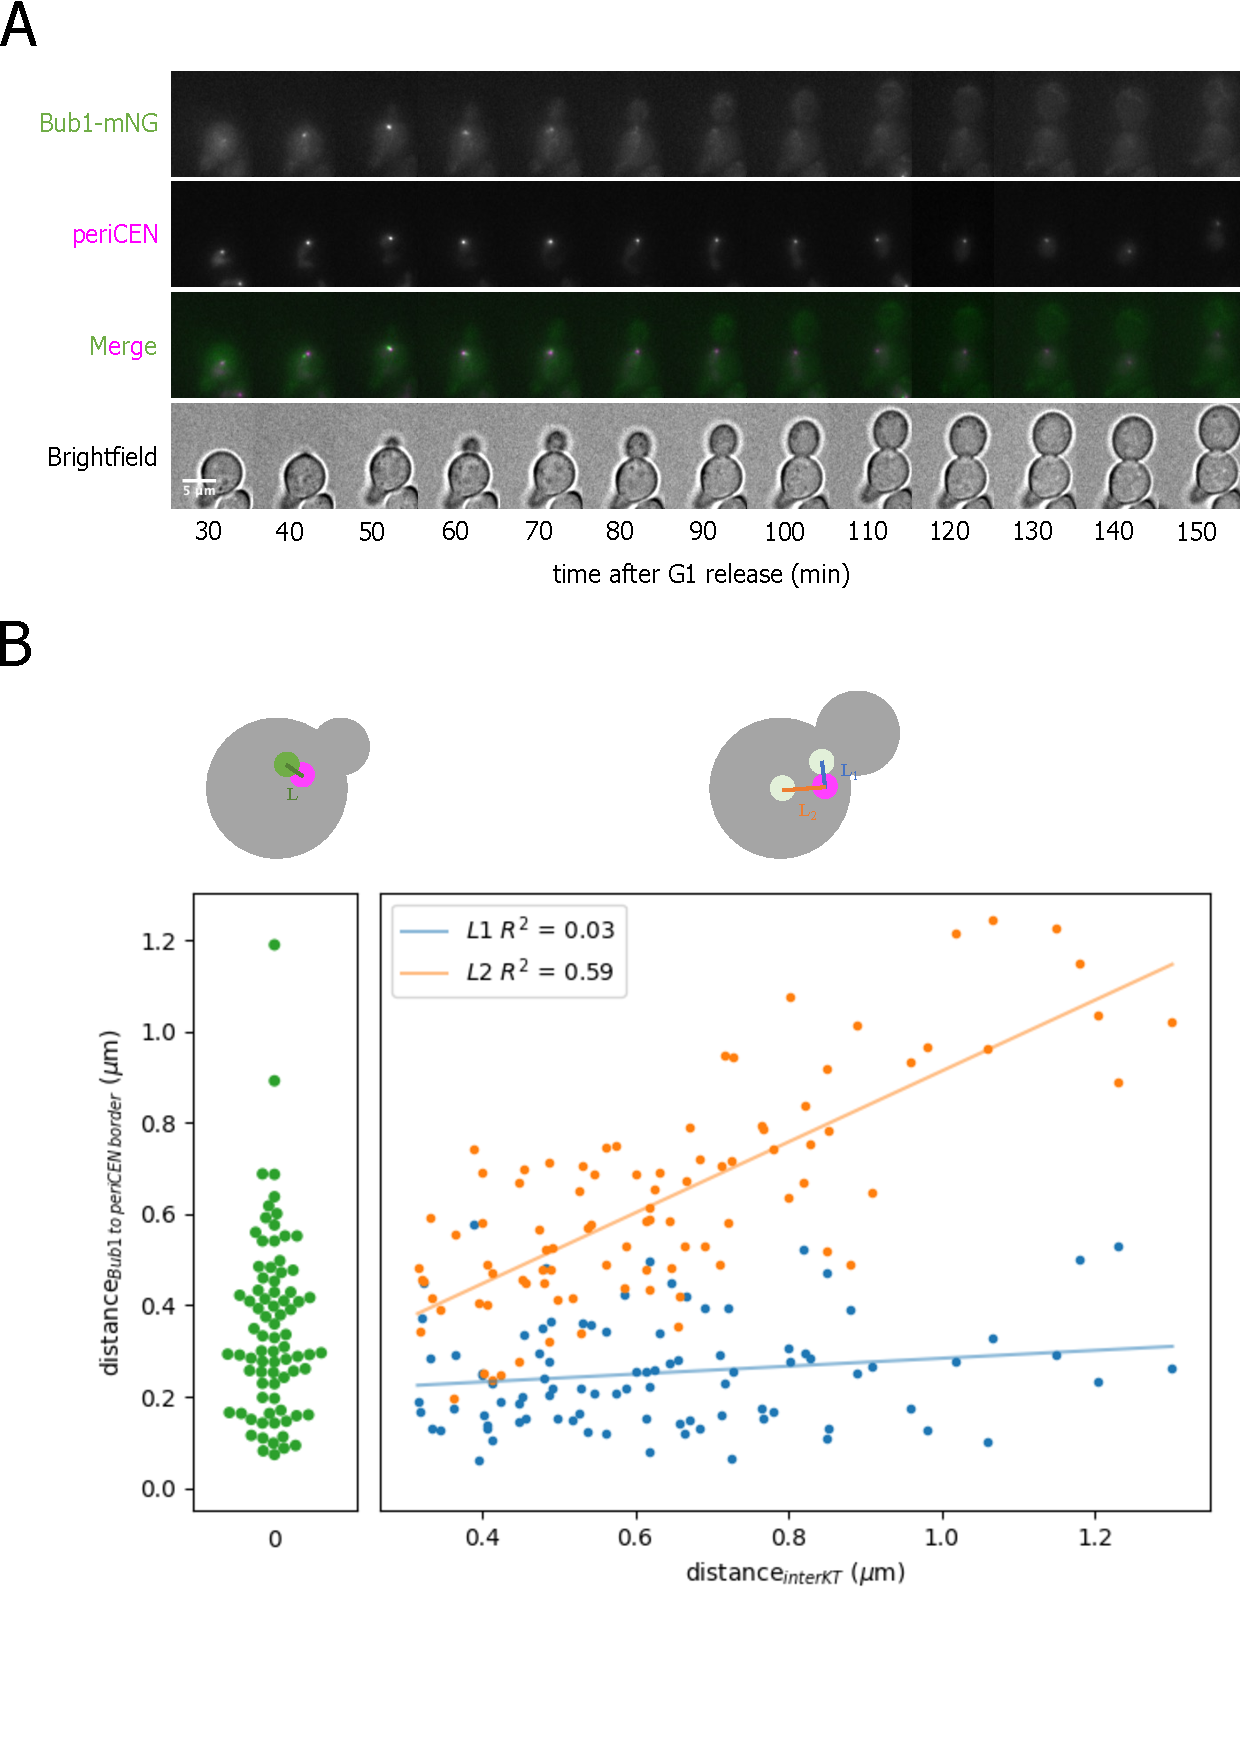
\includegraphics[width=0.9\textwidth]{figures/Bub1-mNG peri-cen.pdf}
  \caption[The shorter distance between Bub1 and peri-centromere is independent of the inter-kinetochore distance]{The shorter distance between Bub1 and peri-centromere is independent of the inter-kinetochore distance. (A) Montage of representative time-lapse imaging. (B) Scatter plot showing the relation of Bub1-to-peri-centromere distance and inter-kinetochore distance. N=30 cells were followed over time and quantified for $L$ (the distance before Bub1-mNG separation), $L_{1}$ (the shorter distance after Bub1-mNG separation) and $L_{2}$ (the longer distance after Bub1-mNG separation), which are presented in green, orange and blue, respectively. The line with the same colour represents the model of simple linear regression. }
  \label{fig:periCEN}
\end{figure} 

\nomenclature{+MET}{methionine-containing}
\nomenclature{-MET}{methionine-depleted}
\nomenclature{mNG}{mNeonGreen}

\subsection{Bub1 is re-localised from the kinetochore by tension}
During data analysis of the previous experiment, I noticed a reduction in fluorescence intensity of Bub1-mNG foci as they separate to an extent that they are barely visible at the end of imaging. This cannot be simply explained by photo-bleaching because tdTomato is supposed to have a shorter bleaching time than mNG, yet it remains visible (Figure~\ref{fig:periCEN}A). The observation raises the possibility that the kinetochore localisation of Bub1 could be under the regulation of tension, leading to the physical separation from its substrates. The idea that Bub1 localisation could be regulated by tension has been implicated in literature \citep{Asai2020, Proudfoot2019, Jin2017PrematureCerevisiae}. To test this, I wanted to quantify the dynamics of the amount of Bub1 at the kinetochore as well as the inter-kinetochore distance. Since Bub1-mNG becomes indistinguishable from the background after separation, I chose to use the outer-kinetochore protein Mtw1 as a more reliable measure of the inter-kinetochore distance. I constructed a strain bearing BUB1-mNG MTW1-tdTomato pMET-CDC20. Time-lapse live-cell imaging was again performed since the G1 release (Figure~\ref{fig:bub1mtw1}A). As expected, Bub1-mNG follows the same dynamics as in the previous experiment. While Mtw1-tdTomato appears as one focus at the start of imaging and then splits into two foci as the cell cycle progresses (Figure~\ref{fig:bub1mtw1}B). Further quantification showed that the fluorescence intensity of kinetochore Bub1-mNG peaks at 60 \si{\minute} since G1 release, with an over 2-fold decrease at 70 \si{\minute}, coinciding with the beginning of Mtw1-tdTomato foci separation (Figure~\ref{fig:bub1mtw1}C). This indicates that kinetochore-localised Bub1 is reduced upon the establishment of bi-orientation. 

\begin{figure}[htbp]
  \centering
  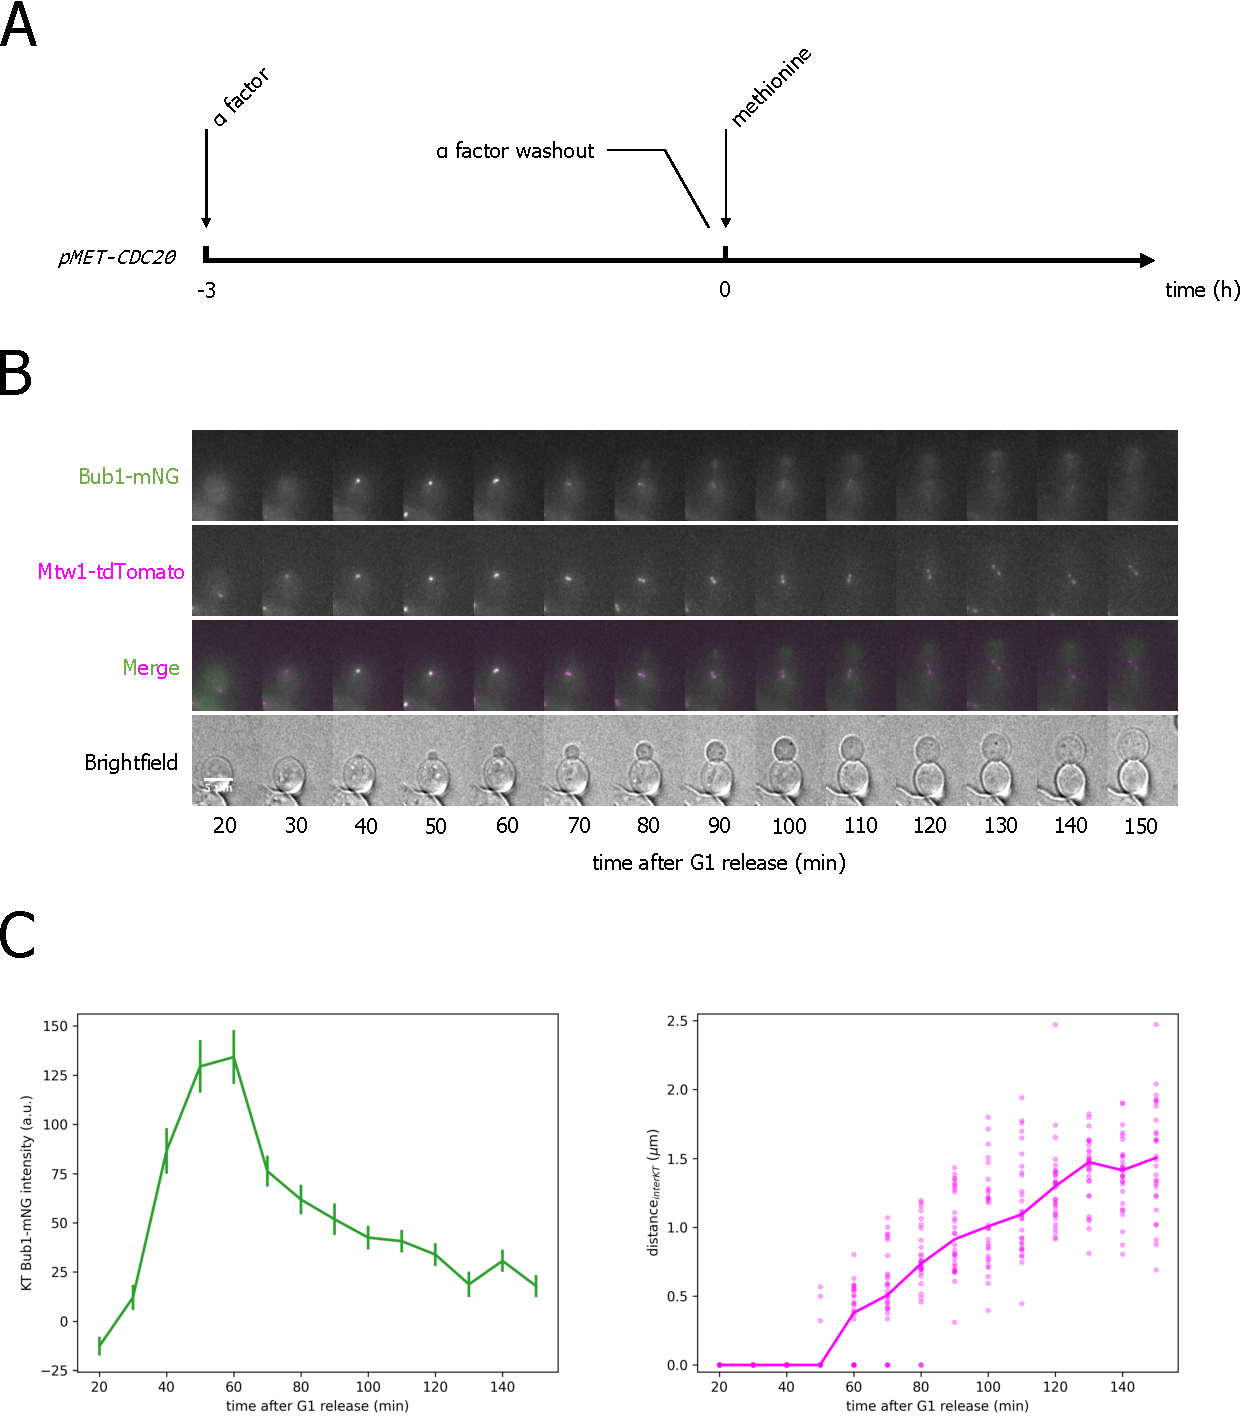
\includegraphics[width=0.9\textwidth]{figures/Bub1-mNG vs Mtw1-td.pdf}
  \caption[Kinetochore-localised Bub1 is reduced upon bi-orientation]{Kinetochore-localised Bub1 is reduced upon bi-orientation. (A) Schematics of experimental procedures. (B) Montage of representative time-lapse imaging. (C) N=30 cells were followed over time and quantified for kinetochore Bub1-mNG fluorescence intensity and inter-kinetochore distance. Left panel: mean fluorescence intensity of Bub1-mNG at the kinetochore as a function of time. The error bar represents the standard error. Right panel: Median inter-kinetochore distance as a function of time. Individual data points are shown as dots. }
  \label{fig:bub1mtw1}
\end{figure} 

I then sought to test whether the reduction in Bub1 kinetochore localisation is due to protein degradation or re-localisation. Human Bub1 is degraded by APC in anaphase \citep{Qi2007KEN-box-dependentComplex/cyclosome} but it is not known in budding yeast. Hence, I performed a synchronised mitotic time course experiment followed by western blotting to check Bub1 protein expression. Cells bearing BUB1-6HA were synchronised in G1 and released into rich media. $\alpha$ factor was added 60 \si{\minute} after the release to arrest cells in the next G1 (Figure~\ref{fig:bub1timecourse}A). Tubulin IF was used to examine the progression of the cell cycle. At 75 \si{\minute} after G1 release, over 80\% of cells were in metaphase while most cells were in anaphase at 90 and 105 \si{\minute} (Figure~\ref{fig:bub1timecourse}B). Western blotting with anti-HA antibody showed Bub1 protein level reached its apex at 90 \si{\minute} and started to decrease since 105 \si{\minute} (Figure~\ref{fig:bub1timecourse}C), suggesting Bub1 is degraded in late anaphase in budding yeast. Therefore, protein degradation could not be the reason for reduced Bub1 kinetochore localisation in metaphase in the previous experiment. Interestingly, Bub1 experienced changes in electrophoretic mobility at the early stage of the cell cycle, indicating its phosphorylation status might be actively regulated. As this is beyond the scope of my project, this was not investigated further. 

\begin{figure}[htbp]
  \centering
  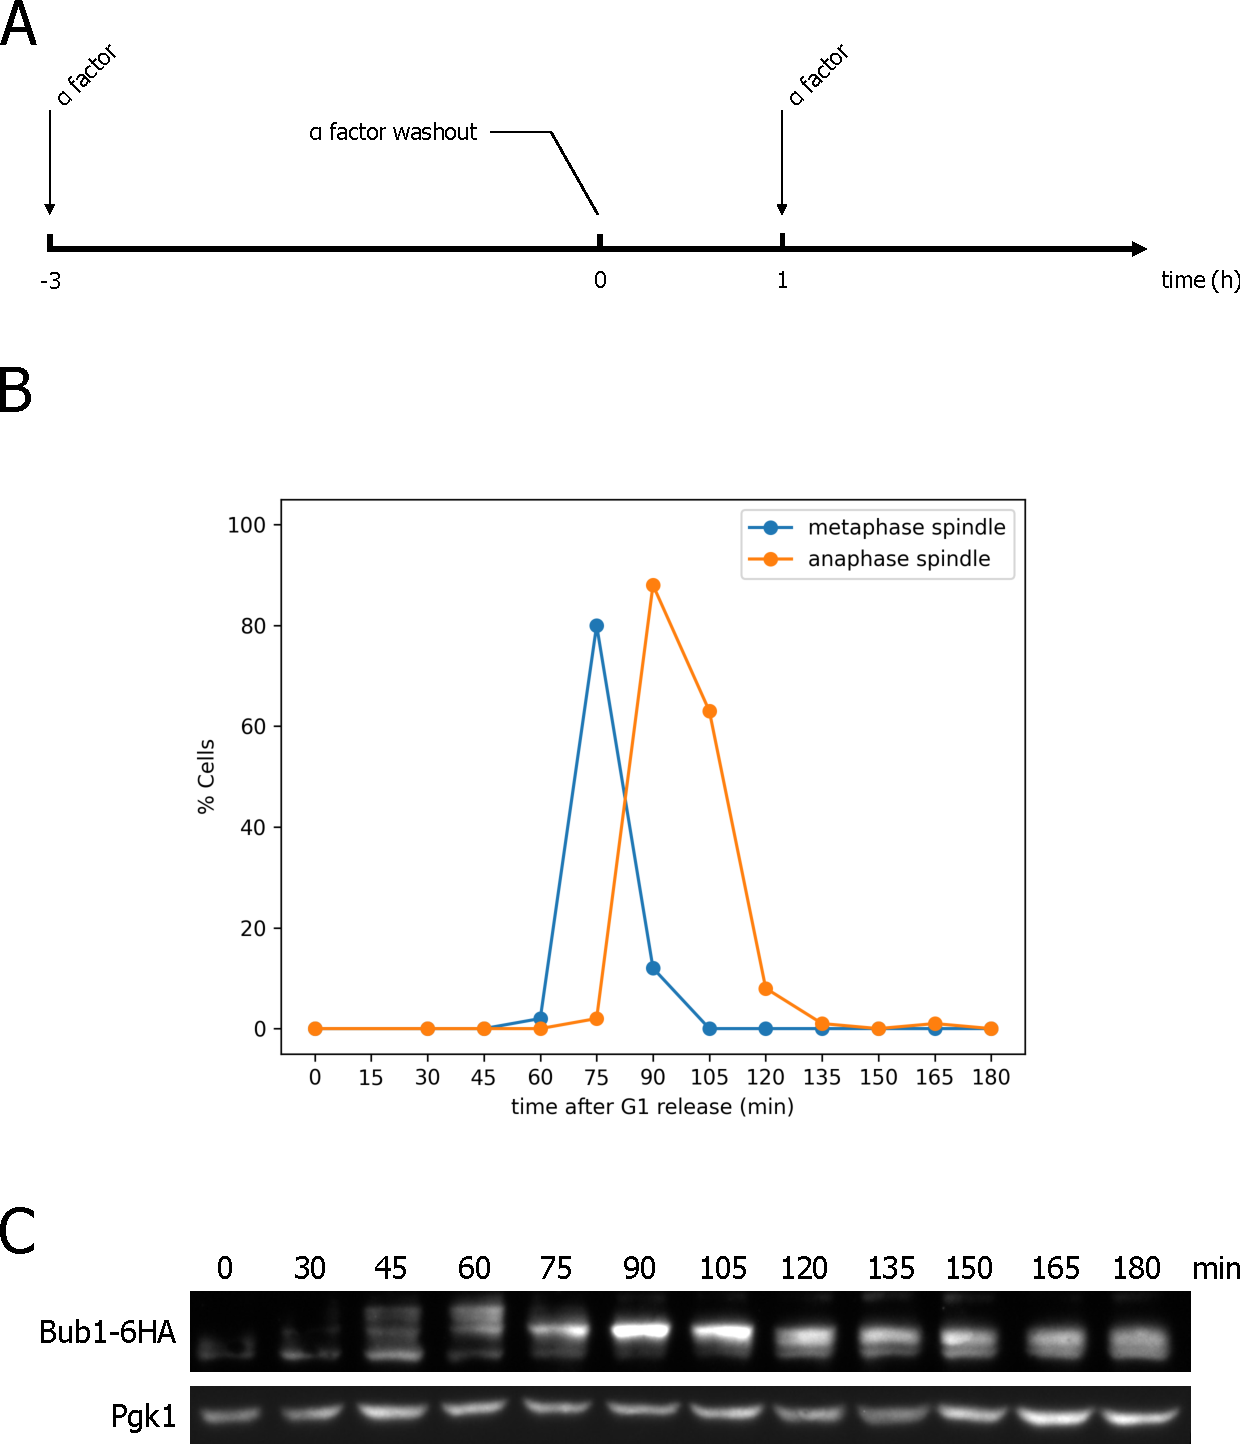
\includegraphics[width=0.9\textwidth]{chapter3/figures/Bub1-6HA time course.pdf}
  \caption[Bub1 is not degraded until anaphase]{Bub1 is not degraded until anaphase. (A) Schematics of experimental procedures. (B) The proportion of cells with metaphase or anaphase spindle over time by tubulin IF. (C) Western blotting with anti-HA antibody to detect Bub1 protein. Pgk1 was used as the loading control.}
  \label{fig:bub1timecourse}
\end{figure} 

The experiments above suggest that Bub1 is re-localised from the kinetochore upon bi-orientation. Given that both tension and kinetochore-microtubule attachment are established in this case, it is not known whether tension is required for Bub1 de-localisation besides attachment. To abolish tension without disrupting attachment, I decided to disable sister chromatid cohesion by depleting the kleisin subunit Scc1 of the cohesin complex. Cells from Figure~\ref{fig:bub1mtw1} with or without additional pMET-SCC1 were synchronised in G1. Methionine was added 45 \si{\minute} before release to pre-clean Scc1 in the pMET-SCC1 strain. Live-cell imaging was performed to quantify kinetochore Bub1-mNG fluorescence intensity and inter-kinetochore distance (Figure~\ref{fig:bub1metscc1}A). As expected, the pMET-SCC1 strain exhibited increased inter-kinetochore distance ($\sim$2.5 \si{\micro\metre} towards the end of the experiment) compared to the wild type ($\sim$1.5 \si{\micro\metre} towards the end of the experiment), indicating a reduction in sister chromatid cohesion. Unlike the wild type, the signal of kinetochore Bub1-mNG is maintained at a similar value after 60 \si{\minute} from G1 release in the pMET-SCC1 strain (Figure~\ref{fig:bub1metscc1}B and C), suggesting Bub1 is not removed from the kinetochore in the absence of tension while no additional disruption was applied on attachment. To rule out the potential artefacts from pMET-SCC1 causing an increase in Bub1 expression, I used western blotting to check the Bub1 protein expression level in the wild type and the pMET-SCC1 strain arrested in metaphase by methionine depletion. No obvious difference was observed (Figure~\ref{fig:bub1metscc1}D). Hence, the kinetochore localisation of Bub1 is reduced by tension. 

\begin{figure}[htbp]
  \centering
  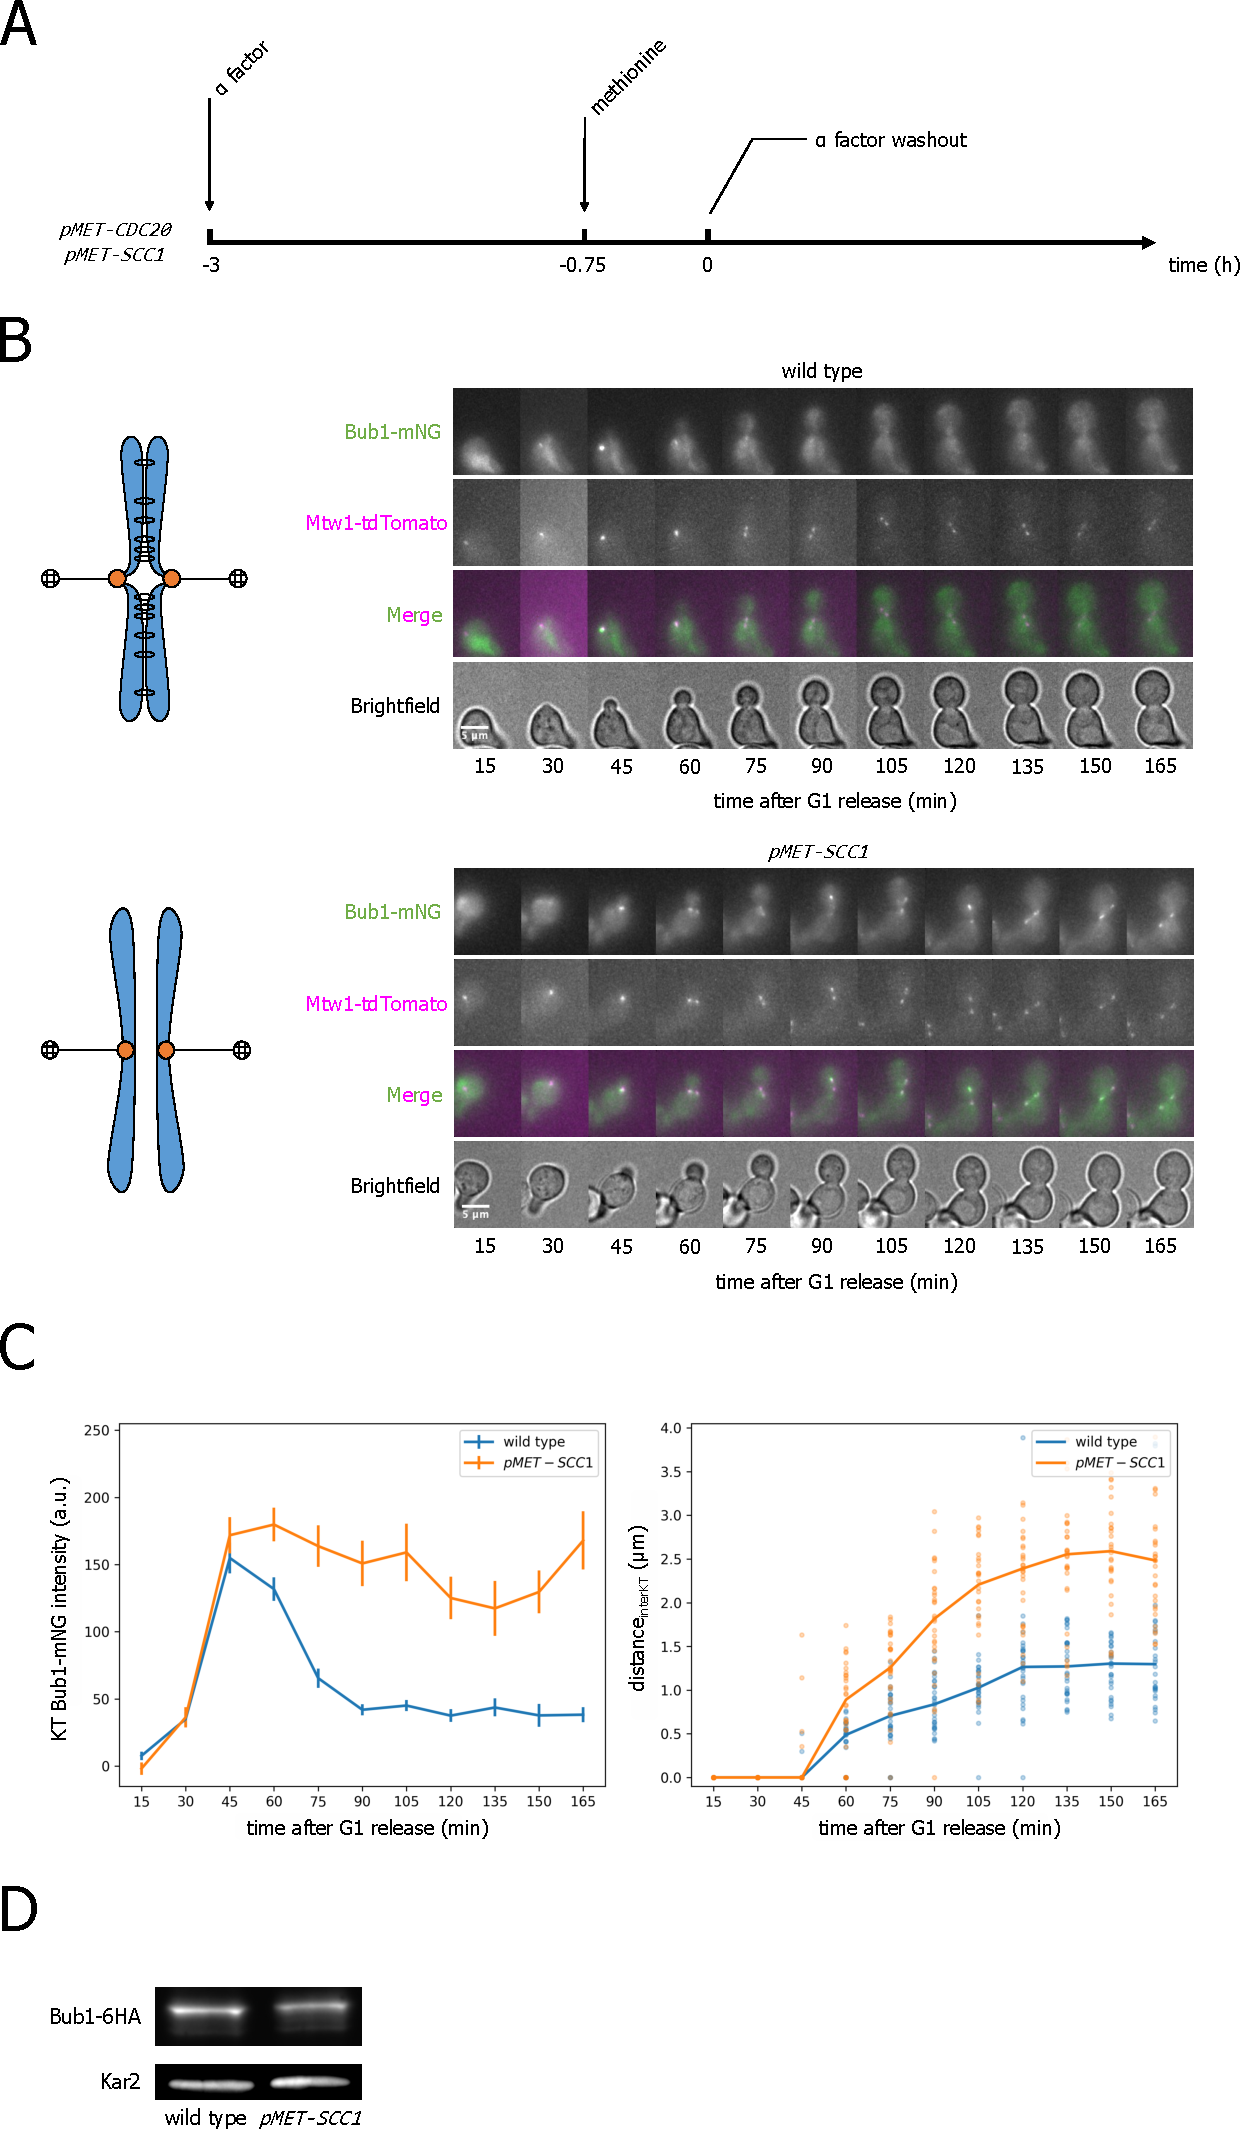
\includegraphics[width=0.9\textwidth]{chapter3/figures/Bub1-mNG pMET-SCC1.pdf}
  \caption[Tension is required for Bub1 re-localisation from the kinetochore]{Tension is required for Bub1 re-localisation from the kinetochore. (A) Schematics of experimental procedures. (B) Montage of representative time-lapse imaging. Cartoons on the left indicate the status of sister chromatids. (C) N=30 cells were followed over time and quantified for kinetochore Bub1-mNG fluorescence intensity and inter-kinetochore distance. Left panel: mean fluorescence intensity of Bub1-mNG at the kinetochore as a function of time. The error bar represents the standard error. Right panel: Median inter-kinetochore distance as a function of time. Individual data points are shown as dots. The wild type is shown in blue and pMET-SCC1 is shown in orange. (D)  Western blotting with anti-HA antibody to detect Bub1 protein. Kar2 was used as the loading control. }
  \label{fig:bub1metscc1}
\end{figure} 

\subsection{Bub1 re-localisation is earlier than Sgo1 re-localisation }
The data so far have suggested a model where Bub1 and Sgo1 re-localise sequentially. If this is true, we would expect a difference in the timing of their removal. To test it, ideally, a strain with the two proteins tagged with fluorescence proteins of different colours should be used. However, none of Bub1 or Sgo1 tagged with various types of RFPs gave good enough signals under our microscope. Instead, I could only image Bub1-mNG and Sgo1-EGFP in two different strains and use the inter-kinetochore distance measured from Mtw1-tdTomato as the internal control for timing. Standard G1 to metaphase live-cell imaging was carried out (Figure~\ref{fig:bub1sgo1}A). 

\begin{figure}[htbp]
  \centering
  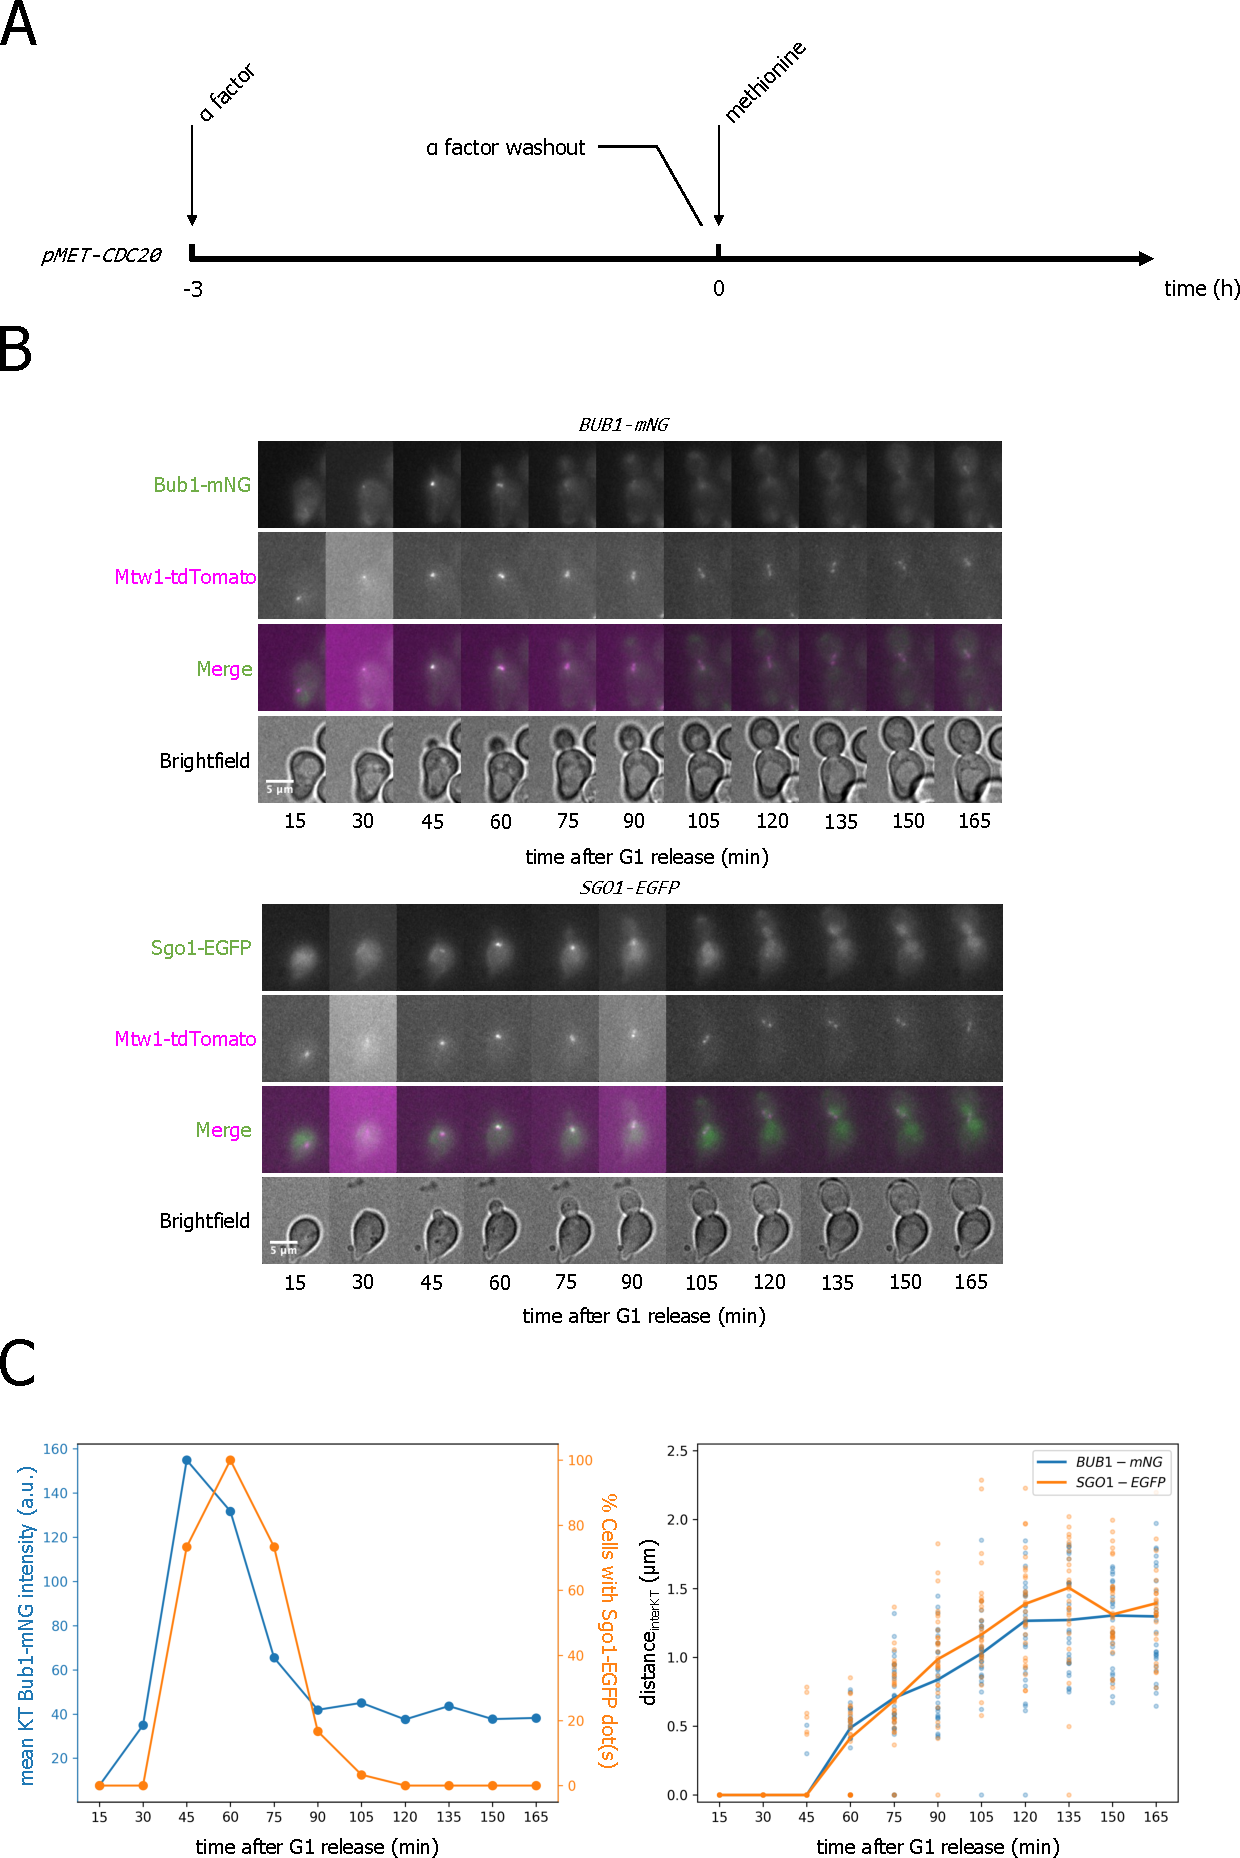
\includegraphics[width=0.9\textwidth]{chapter3/figures/Bub1-mNG Sgo1-EGFP.pdf}
  \caption[Bub1 is re-localised earlier than Sgo1]{Bub1 is re-localised earlier than Sgo1. (A) Montage of representative time-lapse imaging. (B) N=30 cells for each strain were followed over time and quantified. Left panel: mean fluorescence intensity of Bub1-mNG at the kinetochore and percentage of cells with Sgo1 foci as a function of time. Right panel: Median inter-kinetochore distance as a function of time. Individual data points are shown as dots. The BUB1-mNG strain is shown in blue and the SGO1-EGFP strain is shown in orange.}
  \label{fig:bub1sgo1}
\end{figure} 

\section{Discussion}
\section{Materials and methods}
\subsection{Microscopy methods}
\subsubsection{FRET}
The FRET experiment was performed on a Nikon Ti2 inverted microscope equipped with a 100x Plan ApoChromat NA 1.45 oil lens and Prime 95B CMOS (sCMOS) camera. Fluorophores were excited with GFP and emission in the mCherry channel was recorded. Subsequently, standard GFP-GFP and mCherry-mCherry excitation and emission were performed. 

bleed-through from both fluorophores to the FRET channel are subtracted in ImageJ using the following formula: 
Acceptor in FRET channel (Co-efficient A) =	Mean intensity of Acceptor using FRET set/ Mean intensity of Acceptor using acceptor set

Donor in FRET channel (Co-efficient B) = Mean intensity of Donor only using FRET filter set/ Mean intensity of Donor only using Donor filter set

FRET Specimen - (A * FRET Specimen using Acceptor filter set) - (B * FRET Specimen using Donor filter set)

Protocol

Use 3 samples

Acceptor Only
Donor Only
FRET Sample
Collect 5 images

Acceptor Only using Acceptor filter set
Acceptor Only using FRET filter set
Donor Only using Donor filter set
Donor Only using FRET filter set
FRET Specimen Only using FRET filter set

reference \citep{Gordon1998QuantitativeMicroscopy}

\subsubsection{Live-cell imaging}
Cells bearing pMET-CDC20 from patches on -MET plates were inoculated in 10 \si{\milli\litre} of CSM -MET and incubated at RT with shaking at 250 rpm overnight. Cells were diluted to $OD_{600}$=0.2 in 10 \si{\milli\litre} of CSM -MET in the morning, incubating at RT with shaking at 250rpm for over 1 \si{\hour}, allowing cells to enter the exponential phase. Then, cells were re-diluted to $OD_{600}$=0.2 in 10 \si{\milli\litre} of CSM -MET and 10 \si{\micro\litre} of 10 \si{\micro\gram/\milli\litre} alpha factor was added for G1 synchronization. After 1.5 \si{\hour}, another 5 \si{\micro\litre} of 10 \si{\micro\gram/\milli\litre} alpha factor was added. 1.5 \si{\hour} later, shmoo morphology was checked by a light microscope to ensure G1 arrest. 1 \si{\milli\litre} of cell culture was transferred to a 1.5 \si{\milli\litre} Eppendorf tube and concentrated by centrifuging at 3000 rpm for 3 \si{\minute} then removing 700 \si{\micro\litre} of supernatant. 250 \si{\micro\litre} of concentrated cell culture was loaded onto an 8-well Ibidi dish pre-treated with concanavalin A (preparation see separate protocol) and incubated at RT on bench for 15 \si{\minute} to allow cells to bind the bottom of the dish. The supernatant was removed using a bench aspirator and cells were washed twice with 250 \si{\micro\litre} of SC. After the final wash, 250 \si{\micro\litre} of SC was added to each well for imaging. 

\subsubsection{Quantification of fluorescence intensity}

\nomenclature{RT}{Room Temperature}
\nomenclature{rpm}{revolutions per minute}